\chapter{Requirements}
\section{Functional requirements}
\begin{table}[H]
\begin{tabularx}{\linewidth}{lX}
\textbf{FR01} & \textbf{Over the air installation}\\
 & The Android application and the Arduino device should communicate over bluetooth and install an arbitrary application from the Arduino Store in a simple two step process.\\
\textbf{FR02} & \textbf{Easy to use interface}\\
 & The Arduino Store application should be easy to use and easy to understand. It should not be necessary to do anything on the Arduino except for starting it. On startup it should search for nearby bluetooth connections with paired devices.\\
 \textbf{FR03} & \textbf{Example PUIs}\\
 & To demonstrate the Arduino Store (on Android), over the air installation, and the application in action on an Arduino.\\
\textbf{FR04} & \textbf{Validation of Arduino hardware and software}\\
 & The Android application should by default hide Arduino applications in the Arduino Store which are incompatible with the Arduino device depending on memory requirements and connected devices.\\
\end{tabularx}
\caption{Functional Requirements}
\end{table}

\section{Non-functional requirements}
\begin{table}[H]
\begin{tabularx}{\linewidth}{lX}
\textbf{NFR01} & \textbf{Usability}\\
 & Both old and young persons should be able to understand how to use the application and install arduino-apps.\\
\textbf{NFR02} & \textbf{Reliability}\\
 & The application on the Arduino should work and start if rebooted.\\
\textbf{NFR03} & \textbf{Open source}\\
 & The project is under European R\&D project SOCIETIES. All source code will be open source under Apache 2.0 license.\\
\textbf{NFR04} & \textbf{Platform compability}\\
 & Arduino Store should be compatible in Android 2.3 and newer. See FR04 for compatibility for Arduinos.\\
\textbf{NFR05} & \textbf{Extensibility}\\
 & It should be easy to add features and extend this product later. The system should therefore be modular to simplify further development.\\
\end{tabularx}
\caption{Non-functional requirements}
\end{table}

%TODO: Do the latex stuffs so it looks nice.
%TODO: bestemme requirements som skal forsvinne og legges til

\section{Use-Cases}
\begin{figure}[H]
\centering
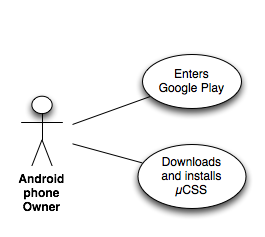
\includegraphics[scale=0.7]{images/UseCase1}
\end{figure}

    \begin{table}[H]
        \begin{tabularx}\linewidth{    |m{0.3 \textwidth} |X|   }
            \hline
                ID           & 1 \\
            \hline
                Name             & Install $\mu$CSS \\
            \hline
                Goal             & Have $\mu$CSS installed on the Android device\\
            \hline
                Actors           & Android device owner\\
            \hline
                Prequisite       & The actor have a Android device with Google Play\\
            \hline
                Main Flow        &  1. Opens Google Play \\
                                 &  2. Search for ``$\mu$C Software Store'' \\
                                 &  3. Installs the application \\
            \hline
                Alternative Flow & None\\
            \hline
                Parent UC        & None\\
            \hline
                Child UC         & All\\
            \hline
        \end{tabularx}
    \end{table}

\begin{figure}[H]
\centering
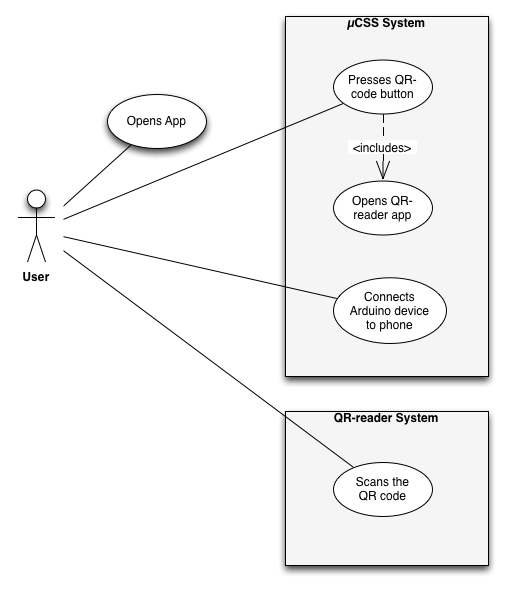
\includegraphics[scale=0.7]{images/UseCase2}
\end{figure}

\begin{table}[H]
    \begin{tabularx}\linewidth{    |m{0.3 \textwidth} |X| }
        \hline
            ID               & 2 \\
        \hline
            Name             & Pair Arduino device and Android device with QR code\\
        \hline
            Goal             & Connect the Arduino device to the Android application with the use of QR code\\
        \hline
            Actors           & Arduino device owner\\
        \hline
            Prerequisite     & Installed $\mu$CSS \\
                             & Installed predefined QR-reader\\
        \hline
            End requirement  & The Arduino device is connected to the phone via bluetooth\\
        \hline
            Main flow        &  1. User opens $\mu$CSS \\
                             &  2. User presses the button indicating that he wants to pair with the Arduino device using QR code \\
                             &  3. The system opens the QR reader application \\
                             &  4. The QR reader application reads the QR code and returns the information it contains\\
                             &  5. The system pairs with the Arduino device \\
        \hline
            Alternative flow &  3.a. The user does not have the right QR code reader installed \\
                             &  3.b. The system prompts the user if he wants to install the QR code reader \\
                             &  3.c. If no: stop \\
                             &  4.a. The QR reader is unable to read the QR code \\
                             &  4.b. Try again or stop\\
        \hline
            Parent UC        & 1\\
        \hline
            Child UC         & 7\\
        \hline
    \end{tabularx}
\end{table}

\begin{figure}[H]
\centering
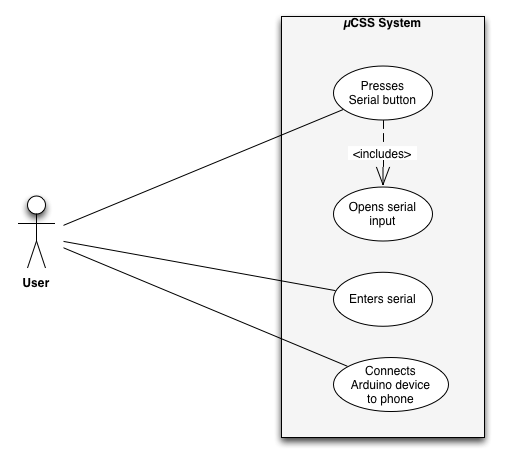
\includegraphics[scale=0.7]{images/UseCase3}
\end{figure}

\begin{table}[H]
    \begin{tabularx}\linewidth{    |m{0.3 \textwidth} |X| }
        \hline
            ID               & 3 \\
        \hline
            Name             & Pair Arduino device with Android device using serial \\
        \hline
            Goal             & Connect the Arduino device to the Android application with the use of QR code \\
        \hline
            Actors           & Arduino device owner \\
        \hline
            Prerequisite     & Installed $\mu$CSS \\
                             & Intstalled predefined QR-reader \\
        \hline
            End requirement  & The Arduino device is connected to the phone via bluetooth \\
        \hline
            Main flow        &  1. User opens $\mu$CSS \\
                             &  2. User presses the button indicating that he
                                    wants to pair with the Arduino device using a serial code \\
                             &  3. System opens dialog box for input\\
                             &  4. The user types the serial \\
                             &  5. The system pairs with the Arduino device \\
        \hline
            Alternative flow &  4.a. The user misspells the serial \\
                             &  4.b. The system displays an error, and prompts again \\
        \hline
            Parent UC        & 1 \\
        \hline
            Child UC         & 7 \\
        \hline
    \end{tabularx}
\end{table}

\begin{figure}[H]
\centering
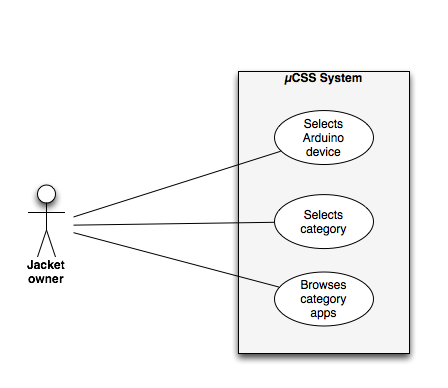
\includegraphics[scale=0.7]{images/UseCase4}
\end{figure}

        \begin{table}[H]
        \begin{tabularx}\linewidth{    |m{0.3 \textwidth} |X| }
            \hline
                ID               & 4 \\
            \hline
                Name             & Browse apps \\
            \hline
                Actors           & Arduino device owner \\
            \hline
                Prequisite       & Installed $\mu$CSS \\
            \hline
                End Requirement  & None \\
            \hline
                Main Flow        &  1. The user opens $\mu$CSS \\
                                 &  2. The user selects the an Arduino device \\
                                 &  3. The user selects category (One category is named ``al'') \\
                                 &  4. The user browses apps \\
            \hline
             Alternative Flow    & 2.a. The user does not select Arduino device, but browses anyway \\
           \hline
        \end{tabularx}
    \end{table}



\begin{figure}[H]
\centering
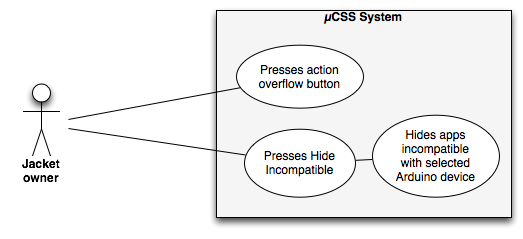
\includegraphics[scale=0.7]{images/UseCase5}
\end{figure}



\begin{figure}[H]
\centering
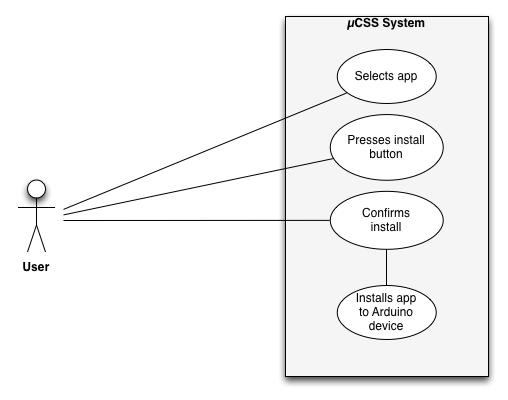
\includegraphics[scale=0.7]{images/UseCase6}
\end{figure}

\begin{table}[H]
    \begin{tabularx}\linewidth{    |m{0.3 \textwidth} |X| }
        \hline
            ID               & 6 \\
        \hline
            Name             & Install application on Arduino device \\
        \hline
            Goal             & Connect the Arduino device to the Android application with the use of QR code \\
        \hline
            Actors           & Arduino device owner \\
        \hline
            Prerequisite     &  Installed $\mu$CSS \\
                             &  Arduino device connected to $\mu$CSS \\
        \hline
            End requirement  & The application is installed on the Arduino device \\
        \hline
            Main flow        &  The user selects the desired application \\
                             &  The user presses the ''install'' button \\
                             &  The user confirms the installation \\
                             &  The application is installed at the Arduino device \\
        \hline
            Alternative flow & none \\
        \hline
            Parent UC        & 1, 2, 3, 4, 5 \\
        \hline
            Child UC         & none \\
        \hline
    \end{tabularx}
\end{table}


\section{Changes in requirements after midterm}
Approaching midterm it was discovered that the over the air transfer of PUI apps to an Arduino device proved to be more demanding than planned. After a extra ordinary meeting with the customer it was decided to change the focus of the assignment. \\
\newline
The goal of the project remained consistent with previous statement. A prototype of the Android store application had been made, though not all functionality was implemented and tested. Further work on the Android application were temporarily put on halt. At this point the resources were primarily focused on implementing the STK500 protocol in Java to allow for programming of Arduino from an Android device. Se below for concrete additions and removals on the requirements.

% Add more as needed
\subsection{Additions}
\paragraph{STK500 protocol} As mentioned above, implementing the STK500 protocol proved more demanding than expected. Initial research done by the group on this area showed that an Java implementation of AVRDude already existed. Further research on the implementation, however, showed that it could not be used as it required programs not available on Android to be installed on the device. As of midterm, implementing the STK500 protocol in Java were added to the requirements.

\subsection{Removals}
\paragraph{$\mu$CSS server component} In agreement with the customer it was decided to remove the server side component of the assignment from the requirements. This was decided in order to pool resources to other, more critical, tasks.

\paragraph{Sync adapter} As the server component of the assignment was removed from the requirements, there was no need for the sync adapter.

